% ============================================================================
% Course Wrap-Up and Outlook
% University of Geneva
% April 20--23 & May 4--7, 2026
% Duration: 25 minutes
% ============================================================================

\documentclass[aspectratio=169,11pt]{beamer}

% ---------- Theme and colors ----------
\usecolortheme{dove}
\setbeamertemplate{navigation symbols}{}
\setbeamertemplate{footline}{%
  \hfill\usebeamerfont{page number in head/foot}%
  \usebeamercolor[fg]{normal text}%
  \insertframenumber\,/\,\inserttotalframenumber\kern1em\vskip4pt}
\setbeamerfont{frametitle}{size=\huge}

% ---------- Packages ----------
\usepackage[utf8]{inputenc}
\usepackage[T1]{fontenc}
\usepackage{amsmath,amssymb,amsfonts}
\usepackage{bm}
\usepackage{graphicx}
\graphicspath{{fig/}}
\usepackage{tikz}
\usetikzlibrary{shapes,arrows.meta,positioning,calc,fit,backgrounds,patterns,decorations.pathreplacing}
\usepackage{booktabs}
\usepackage{hyperref}
\usepackage{xcolor}

% ---------- Custom colors ----------
\definecolor{uzhblue}{rgb}{0,0,0.5}
\definecolor{uzhgreylight}{RGB}{236,238,241}
\definecolor{uzhgreydark}{RGB}{81,86,94}
\definecolor{harvardcrimson}{RGB}{153,0,0}
\definecolor{unil@blue}{RGB}{0,140,204}
\definecolor{unil@black}{RGB}{35,31,32}
\definecolor{darkgreen}{RGB}{0,100,0}
\definecolor{darkred}{RGB}{139,0,0}
\definecolor{softblue}{RGB}{70,130,180}
\definecolor{softorange}{RGB}{230,159,0}
\definecolor{softgreen}{RGB}{0,158,115}

% ---------- Set beamer colors ----------
\setbeamercolor{frametitle}{bg=uzhgreylight, fg=uzhblue}
\setbeamercolor{title}{fg=uzhblue}
\setbeamercolor{structure}{fg=uzhblue}
\setbeamercolor{block title}{bg=unil@blue, fg=white}
\setbeamercolor{block body}{bg=uzhgreylight}
\setbeamercolor{block title alerted}{bg=darkred,fg=white}
\setbeamercolor{block body alerted}{bg=red!5}
\setbeamercolor{block title example}{bg=darkgreen,fg=white}
\setbeamercolor{block body example}{bg=green!5}
\setbeamercolor{item}{fg=unil@black}
\setbeamercolor{normal text}{fg=unil@black}

% ---------- Emphasis and hyperlinks ----------
\newcommand{\emphc}[1]{\textcolor{harvardcrimson}{#1}}
\hypersetup{colorlinks,linkcolor=harvardcrimson,urlcolor=harvardcrimson}

% ---------- Math commands ----------
\newcommand{\R}{\mathbb{R}}
\newcommand{\E}[1]{\mathbb{E}\!\left[#1\right]}

% ---------- Title ----------
\title[Deep Learning -- Geneva 2026]%
{Deep Learning for Economics and Finance}
\subtitle{Course Wrap-Up and Outlook}
\author{Simon Scheidegger}
\institute[HEC Lausanne]{HEC, University of Lausanne}
\date{University of Geneva\\April 20--23 \& May 4--7, 2026}

\begin{document}

% --- Slide 1: Title ---
{\setbeamercolor{background canvas}{bg=uzhgreylight}
\begin{frame}
\titlepage
\vspace{-0.4cm}
\begin{center}
{\footnotesize Closing lecture for Day 8: climate economics, deep UQ, and policy design}\\[4pt]
{\footnotesize Materials: \url{https://github.com/sischei/Deep_Learning_for_Solving_And_Estimating_Dynamic_Economic_Models}}
\end{center}
\end{frame}
}

% --- Slide 2: Wrap-up roadmap ---
\begin{frame}{Wrap-Up Roadmap (25 min)}
\begin{enumerate}
    \item \textbf{Synthesis of the full course pipeline} (8 min)
    \item \textbf{Decision guide: DEQN, PINN, Surrogates, GP} (7 min)
    \item \textbf{Day 8 lessons for climate-policy modeling} (6 min)
    \item \textbf{Implementation checklist and outlook} (4 min)
\end{enumerate}
\end{frame}

% --- Slide 3: Big picture ---
\begin{frame}{The Big Picture: One Computational Paradigm}
\begin{center}
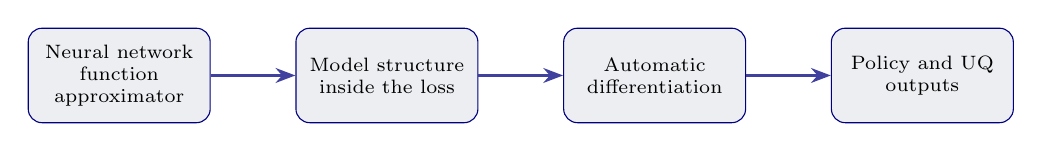
\begin{tikzpicture}[
    box/.style={rectangle, draw=uzhblue, fill=uzhgreylight, rounded corners=5pt,
                text width=2.1cm, minimum height=1.2cm, align=center, font=\scriptsize,
                inner sep=3pt},
    arr/.style={-{Stealth[length=2.5mm]}, very thick, uzhblue!75}
]
\node[box] (nn)     at (0,0)    {Neural network\\function approximator};
\node[box] (loss)   at (3.4,0)  {Model structure\\inside the loss};
\node[box] (ad)     at (6.8,0)  {Automatic\\differentiation};
\node[box] (policy) at (10.2,0) {Policy and UQ\\outputs};

\draw[arr] (nn.east)   -- (loss.west);
\draw[arr] (loss.east) -- (ad.west);
\draw[arr] (ad.east)   -- (policy.west);
\end{tikzpicture}
\end{center}

\vspace{0.25cm}
\begin{block}{Across methods}
DEQN, PINN, deep surrogates, and GP-BAL differ in objective and geometry,\\
but share the same core optimization logic.
\end{block}
\end{frame}

% --- Slide 4: Course arc ---
\begin{frame}{Course Arc: Day 1 to Day 8}
\small
\begin{center}
\begin{tabular}{ll}
\toprule
\textbf{Day} & \textbf{Core step in the pipeline} \\
\midrule
1 & Deep learning foundations and optimization diagnostics \\
2--4 & DEQNs for discrete-time equilibrium (RA, IRBC, OLG, heterogeneity) \\
5 & PINNs for continuous-time PDE problems \\
7 & Deep surrogates and GP/BAL for fast policy/estimation loops \\
8 & Climate IAMs, deep UQ, constrained policy design \\
\bottomrule
\end{tabular}
\end{center}

\vspace{0.2cm}
\begin{alertblock}{Main message}
The toolkit is modular: solve, emulate, quantify uncertainty, then optimize policy under explicit constraints.
\end{alertblock}
\end{frame}

% --- Slide 4b: Visual course timeline ---
\begin{frame}{Visual Timeline of the Course Workflow}
\begin{center}
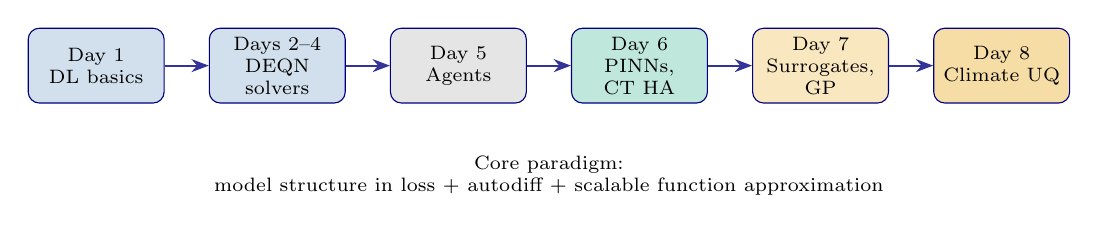
\begin{tikzpicture}[
    phasebox/.style={rectangle, draw=uzhblue, rounded corners=4pt, text width=1.55cm,
                 minimum height=0.95cm, align=center, fill=uzhgreylight, font=\scriptsize,
                 inner sep=2.5pt},
    arr/.style={-{Stealth[length=2.2mm]}, thick, uzhblue!80}
]
\node[phasebox, fill=softblue!25]   (d1) at (0,0)    {Day 1\\DL basics};
\node[phasebox, fill=softblue!25]   (d2) at (2.3,0)  {Days 2--4\\DEQN solvers};
\node[phasebox, fill=gray!20]       (d5) at (4.6,0)  {Day 5\\Agents};
\node[phasebox, fill=softgreen!25]  (d6) at (6.9,0)  {Day 6\\PINNs, CT HA};
\node[phasebox, fill=softorange!25] (d7) at (9.2,0)  {Day 7\\Surrogates, GP};
\node[phasebox, fill=softorange!35] (d8) at (11.5,0) {Day 8\\Climate UQ};

\draw[arr] (d1.east) -- (d2.west);
\draw[arr] (d2.east) -- (d5.west);
\draw[arr] (d5.east) -- (d6.west);
\draw[arr] (d6.east) -- (d7.west);
\draw[arr] (d7.east) -- (d8.west);

\node[font=\scriptsize, align=center] at (5.75,-1.4) {Core paradigm:\\model structure in loss + autodiff + scalable function approximation};
\end{tikzpicture}
\end{center}
\end{frame}

% --- Slide 5: Method decision guide ---
\begin{frame}{Decision Guide: Which Method When?}
\scriptsize
\begin{center}
\begin{tabular}{p{0.16\textwidth}p{0.30\textwidth}p{0.30\textwidth}}
\toprule
\textbf{Method} & \textbf{Use case} & \textbf{Strength} \\
\midrule
DEQN & Discrete-time equilibrium systems & Scales to high-dimensional states \\
PINN & Continuous-time PDE/HJB/KFE systems & Mesh-free PDE residual training \\
Deep surrogate & Repeated model evaluations & Very fast policy and estimation loops \\
GP + BAL & UQ and active design & Built-in uncertainty and sample efficiency \\
\bottomrule
\end{tabular}
\end{center}
\end{frame}

% --- Slide 6: Day 8 contributions ---
\begin{frame}{Day 8 in One Slide}
\textbf{Day 8 in context.}  Pseudo-states let one trained DEQN answer policy questions for \emph{all} plausible parameter values simultaneously.  A GP surrogate on top enables fast computation of SCC, temperature paths, and welfare across the parameter space.  Bayesian active learning then identifies which parameters drive policy recommendations, for example, climate sensitivity matters more than the pure rate of time preference for carbon-tax design.

\vspace{0.25cm}
\begin{exampleblock}{The payoff}
Constrained Pareto-improving tax rules become feasible once the expensive solves are amortized.
\end{exampleblock}
\end{frame}

% --- Slide 7: Failure modes ---
\begin{frame}{Common Failure Modes and Mitigations}
\small
\begin{columns}[T]
\column{0.49\textwidth}
\textbf{Failure modes}
\begin{itemize}
    \item Calibration mismatch to benchmark science
    \item Training focused on wrong state regions
    \item Over-reliance on mean loss diagnostics
    \item Surrogate extrapolation outside training support
\end{itemize}

\column{0.49\textwidth}
\textbf{Mitigations}
\begin{itemize}
    \item Explicit benchmark tests and stress scenarios
    \item Mixed exogenous/endogenous sampling
    \item Report residual distributions and constraints
    \item Active learning and uncertainty-aware evaluation
\end{itemize}
\end{columns}
\end{frame}

% --- Slide 7b: Risk-priority matrix ---
\begin{frame}{Representative Constraint and Uncertainty Results}
\begin{columns}[T]
\column{0.49\textwidth}

\includegraphics[width=\linewidth]{shapley_S1st_GP_E_scc2100.pdf}

\column{0.49\textwidth}

\includegraphics[width=\linewidth]{pareto_frontier_lin_E.png}
\end{columns}

\vspace{0.15cm}
\footnotesize
Left: SCC uncertainty decomposition (Friedl et al., 2023). Right: constrained policy frontier (K\"ubler, Scheidegger, and Surbek, 2025, arXiv:2507.01704).
\end{frame}

% --- Slide 8: Reproducibility checklist ---
\begin{frame}{Implementation Checklist}
\small
\begin{enumerate}
    \item Define state/control vectors and feasibility transforms.
    \item Engineer residual blocks from economics and climate equations.
    \item Set sampling scheme and training diagnostics before tuning architecture.
    \item Validate on out-of-sample simulations and benchmark moments.
    \item Build surrogate/UQ layer only after solver quality is verified.
    \item Separate normative objective from political/participation constraints.
\end{enumerate}
\end{frame}

% --- Slide 9: Frontier directions ---
\begin{frame}{Research Frontier}
\begin{itemize}
    \item Richer heterogeneity: regional, sectoral, and household dimensions.
    \item Endogenous innovation and technology diffusion under climate policy.
    \item Multi-model and model-ensemble learning for robust policy design.
    \item Tight integration of Bayesian learning and policy commitment under ambiguity.
    \item Better theoretical guarantees for convergence and error bounds.
\end{itemize}
\end{frame}

% --- Slide 10: Reading map ---
\begin{frame}{Reading and Notebook Map}
\small
\textbf{Day 8 readings}
\begin{itemize}
    \item \texttt{lectures/day8/readings/CDICE\_Restud\_production.pdf}
    \item \texttt{lectures/day8/readings/CDICE\_Restud\_production\_appendix.pdf}
    \item \texttt{lectures/day8/readings/DeepUQ\_with\_an\_application\_to\_IAM.pdf}
    \item \texttt{lectures/day8/readings/JPE\_Macro.pdf}
\end{itemize}

\vspace{0.2cm}
\textbf{Day 8 notebooks} (suggested order)
\begin{itemize}
    \item \texttt{01\_Climate\_Exercise.ipynb} \hfill (NumPy warm-up: carbon cycle, damages, BAU vs mitigation)
    \item \texttt{02\_DICE\_DEQN\_Library\_Port.ipynb} \hfill (deterministic CDICE-DEQN, library port)
    \item \texttt{03\_Stochastic\_DICE\_DEQN.ipynb} \hfill (AR(1) shocks, Gauss--Hermite, SCC fan charts)
\end{itemize}
\end{frame}

% --- Slide 11: Closing ---
\begin{frame}{Closing Message}
\begin{block}{From method to policy}
Deep learning methods are most useful when they improve \emphc{economic credibility},
\emphc{computational scalability}, and \emphc{policy transparency} at the same time.
\end{block}

\vspace{0.5cm}
\begin{center}
{\Large Thank you for participating in the course.}\\[6pt]
{\LARGE \emphc{Questions and discussion}}
\end{center}
\end{frame}

\end{document}
